\section{INITIAL RESEARCH \hrulefill}

The purpose of the initial project research phase is to enable early
identification of risks, design decisions, and other factors which will
contribute to the creation of the project plan.

\subsection{Analysis of the Dataset}

In order to determine the technical scope of the project it is necessary to
analyse the dataset which the web service will house. The dataset was supplied
by Dr. Flower in the form of a Microsoft Excel spreadsheet consisting of a
single table with 5,773 unique rows over 22 columns. In order to develop a
relational model for this data, each of the 22 unique columns can be considered
as a set of attributes A1,A2,…,A22 and combined to form a relational schema R
(Figure 2 shows this schema with attribute names taken from the spreadsheet
column headings), with the spreadsheet values forming an instance of this
relation r(R) in which each row can be considered a set of tuples where t' =
{t'(A1),t'(A2),…,t'(A22)} ϵ r(R).

\begin{figure}[H]
\centering
\begin{quote}
\textit{R = \{Origin, EC, Protein, Alternative name(s), Source, Organ and/or
  Subcellular locaction, M.W, No., M.W2, No. of Iso-enzymes, pI maximum value,
  pI Min Value, pI Max Value, pI value of major component, pI, Temperature (oC),
  Method, Valid sequence(s) available, UniportKB/ Swiss-Prot/ Protein sequence,
  Species Taxonomy, Full text, Abstract only, Pubmed, Notes\}}
\end{quote}
\caption{A formal relation schema with named attributes}
\label{fig:formal-schema-names-attributes}
\end{figure}

Each tuple represents a single recording of experimentally-derived data, which
lists the origin of the record (such as a research paper, or academic journal),
and 21 attributes which describe the properties of the protein, the experimental
result and the method used to derive it, and links to relevant online
resources. Figure 3 shows a breakdown of the different origins for all of the
records. In order to aid in the design of the database which will be used to
store this dataset, a dataset analysis tool was developed which parses the
dataset file and extracts and derives key information about its properties, and
this information can be used to help determine the best method to use when
storing this data.

\begin{figure}[H]
\centering
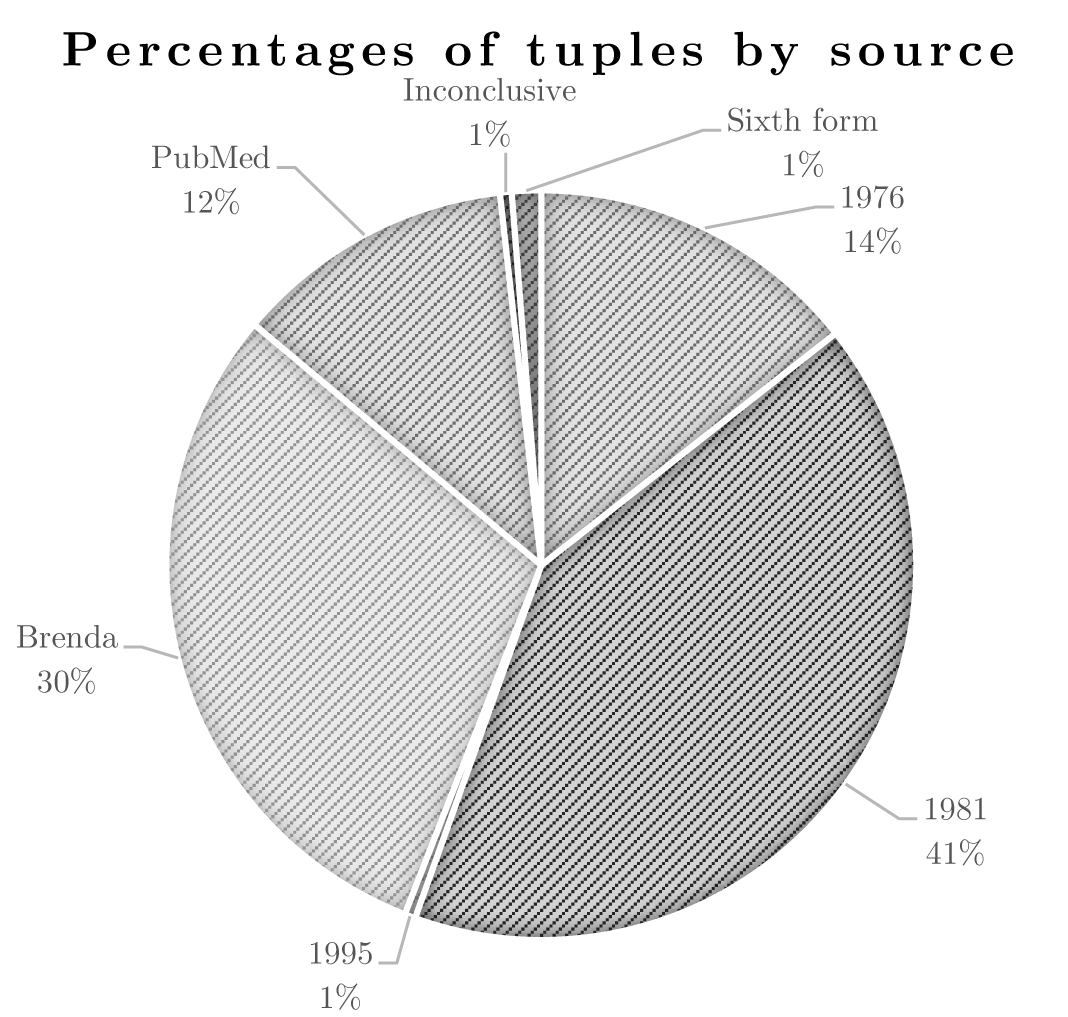
\includegraphics{assets/chart-dataset-origin.png}
\caption{A breakdown of the tuple origins within the dataset}
\label{fig:chart-dataset-origin}
\end{figure}

\newpage
\begin{figure}[H]
\centering
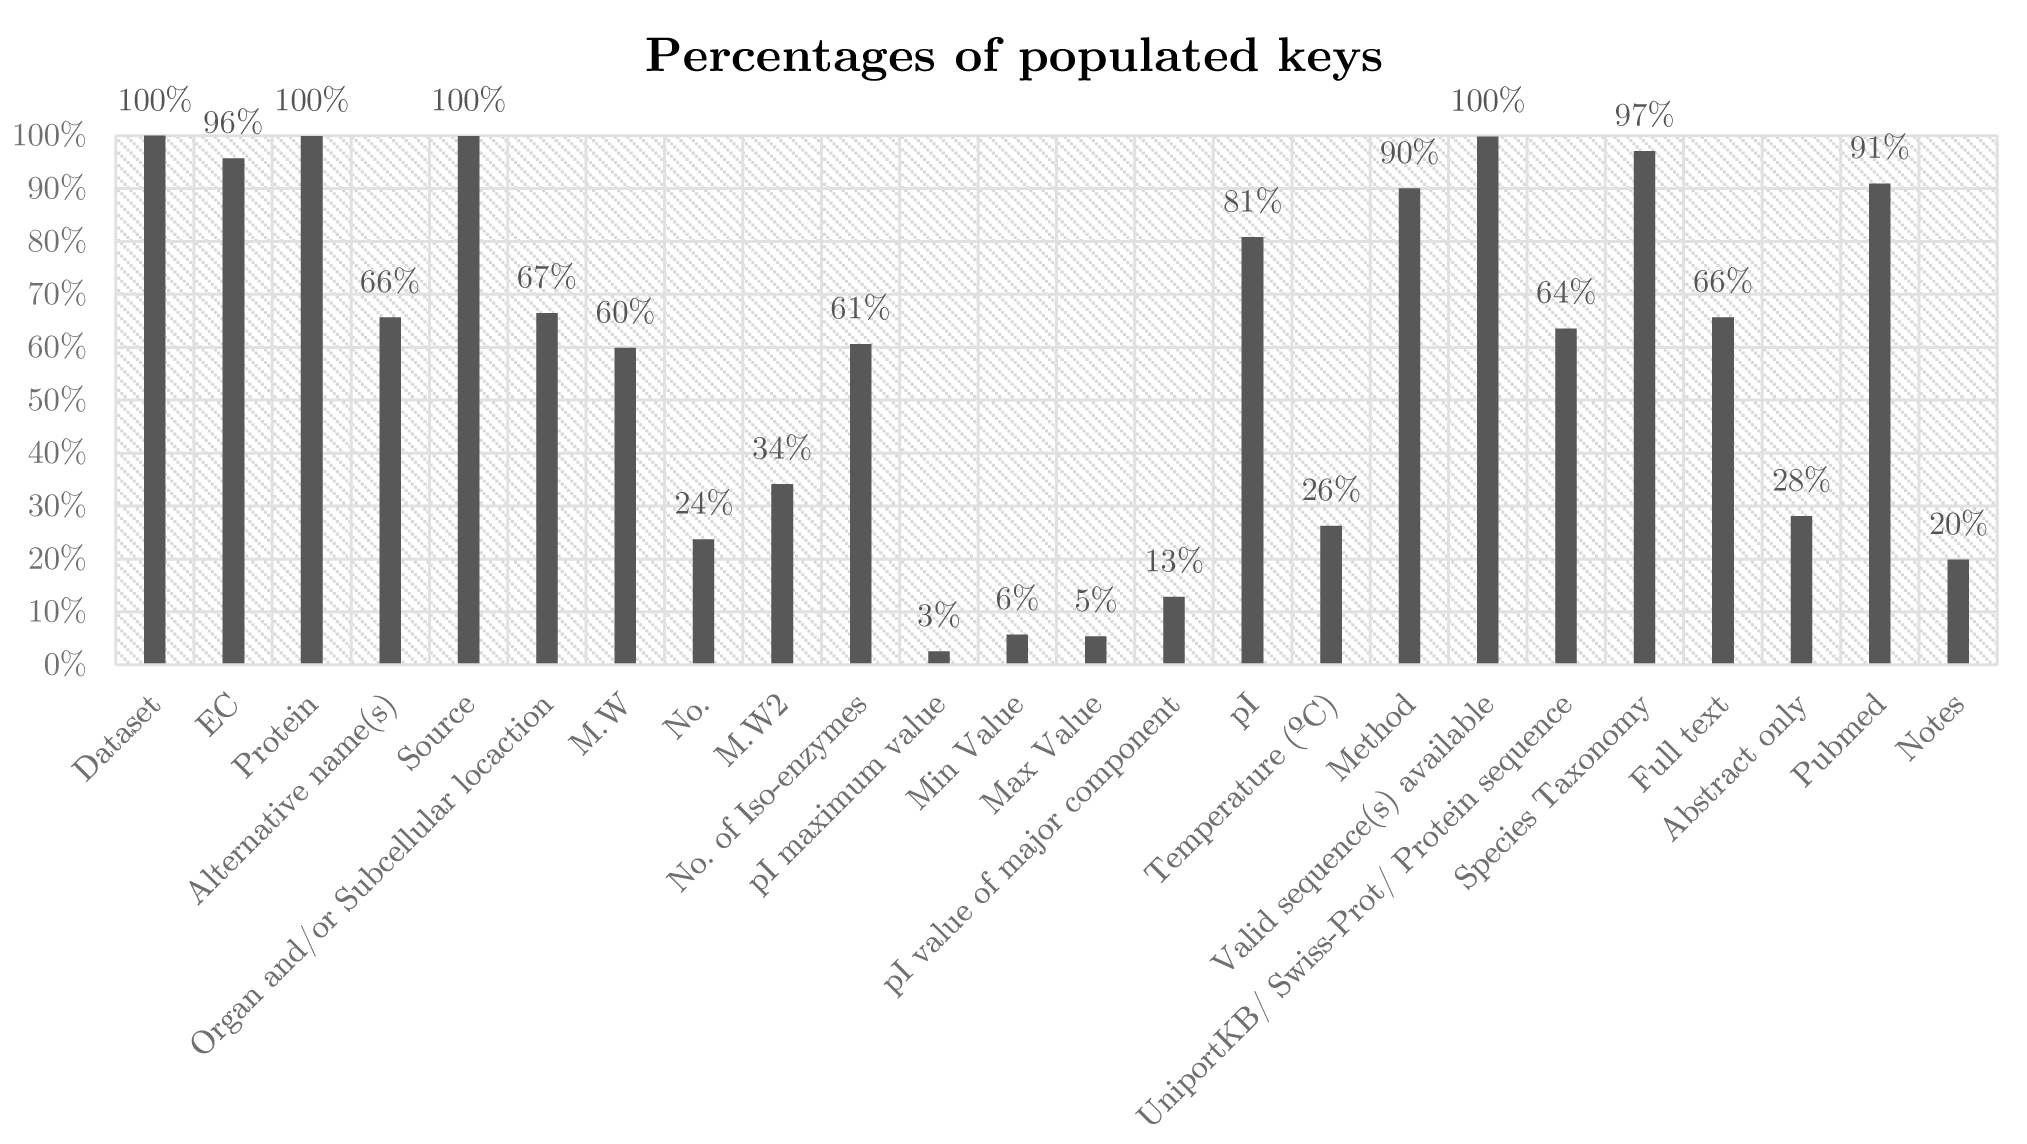
\includegraphics{assets/chart-dataset-populated.png}
\caption{The number of populated keys for each tuple within the dataset}
\label{fig:chart-dataset-populated}
\end{figure}

This early dataset analysis highlighted a number of properties which will
greatly influence the design of the database backend. Chiefly, that the dataset
contains a large number of duplicate keys, and for each tuple, many of the keys
may not be given. This information will have a great influence on the design of
the database; for example, the low percentage of unique values for many of the
records in the dataset indicate that a 3NF normalisation pattern could be used
to gain maximum size efficiency of the stored database \cite{Maier1983}, and so
time should be allocated in project plan to allow for database design decisions
to be investigated and tested.

\begin{figure}[H]
\centering
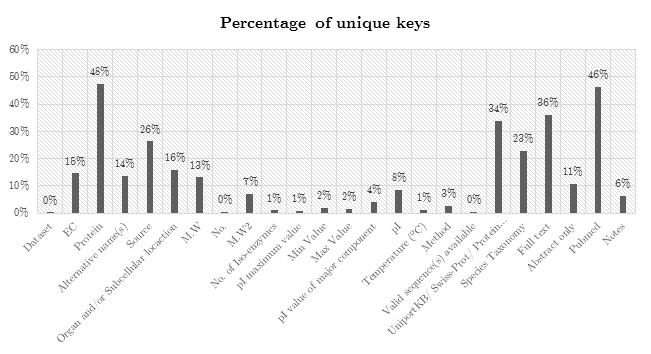
\includegraphics{assets/chart-dataset-unique.png}
\caption{The number of unique keys for each tuple within the dataset}
\label{fig:chart-dataset-unique}
\end{figure}

\newpage
\subsection{Related Bioinformatics Databases}
In addition to gaining a greater understanding of the provided dataset, a
selection of relevant existing websites and databases were examined, in order to
help analyse the strengths and weaknesses of each. As previously stated,
biological databases of protein properties abound, and Dr. Flower's
bioinformatics research has led to the creation of three such databases:
AntiJen, DSD, and PPD:

\paragraph{AntiJen} a kinetic, therm odynam ic and cellular database
\cite{DDG1999}. AntiJen is a database containing quantitative binding data for
peptides. The database houses over 24,000 entries from published experimentally
determined data, and offers keyword searching of this dataset, with results
being returned in a tabular format.

\paragraph{DSD} A database of dehydrogenase stereospecificities
\cite{DDGND}. DSD offers a similar set of features as AntiJen but for a
different dataset. In addition to keyword searching, the website supports
viewing data by selecting from categories, and additionally offers BLAST
searching, which is a feature that will incorporated into this project.

\paragraph{PPD} Protein pKa Database \cite{DDGNDa}. PPD offers data lookup by
either BLAST search or a detailed search page which allows the user to select
from a given set of criteria, such as protein name, experimental method, and
amino acid name.\\

In each of the websites, a large dataset of very specific biological data is
hosted on a website which offers a service for members of the public to query
certain aspects of it and return results. In each case, it is only possible to
return a reduced subset of the data, with no ability for users to download the
entire set in one go; the idea being that users should be allowed to answer
specific queries they may have, but not to idly download the entire dataset
which may be the result of many years of researcher's work. From a technical
standpoint, the websites appear lacking in some areas such as user interface
design, where their rather dated aesthetic and design leads to a rather poor
user experience. Of course this has no bearing on the usefulness of the service
and data offered by the websites, but a greater level of ease of use and control
over the format in which search results are displayed could lead to a more
engaging experience for the user, as well as allowing them to attain the data
they need in a more efficient manner.

\subsection{Previous Final Year Project Analysis}

In addition to the existing public bioinformatics databases which Dr. Flower
assisted in creating, students from previous years have attempted to develop a
similar project to this one. Chief among these was an earlier implementation of
a protein isoelectric point database, created by former student Mohammad
Abdullah. The project used an older and reduced-size version of the current
dataset, and used a MySQL database to store the data, with a PHP back-end to
query the tables and generate static HTML webpages which can be served over an
Apache webserver. A technical review of the implementation revealed a number of
things that could be improved upon – largely that the codebase is a somewhat
impenetrable mixture of PHP with inline HTML, with no distinction between the
application logic and presentation tier, and the querying mechanism is quite
primitive, with little ability to perform advanced searching within the
dataset. Appendix B (page 17) contains a UML diagram of the database schema
used, which highlights the small number of tables used, with few relational
links between records leading to a simplistic searching mechanism.
